%\documentclass[a4paper,
%%twocolumn
%]{article}
\documentclass[a4paper,9pt]{extarticle}

%%%%  Math
\usepackage{amsmath}
\DeclareMathOperator*{\argmin}{argmin}
\DeclareMathOperator*{\argmax}{argmax}
\newcommand*{\argminl}{\argmin\limits}
\newcommand*{\argmaxl}{\argmax\limits}

%%%%  Page margins
\usepackage{geometry}
%\geometry{left=25mm, right=20mm, top=30mm, bottom=20mm}
%\geometry{left=32mm, right=29mm, top=35mm, bottom=23mm}
\geometry{left=36mm, right=32mm, top=35mm, bottom=30mm}
%\geometry{left=15mm, right=15mm, top=25mm, bottom=20mm}
%\setlength{\columnsep}{4.5mm}

%%%% Configuration file for plotting
%%%%%%  Math
\usepackage{amsmath}
\usepackage{amssymb}

%%%%%%  Tables
\usepackage{booktabs}
% \usepackage{longtable}
\usepackage{multirow}
\usepackage{pgfplotstable}
\DeclareMathVersion{sansserif}
\SetSymbolFont{operators}{sansserif}{OT1}{cmss}{m}{n}
\usepackage{siunitx} 
\sisetup{group-separator={,}, group-minimum-digits={3}, parse-numbers=false}
\usepackage{tabularx}
\usepackage{ltablex}
\usepackage{array}
\newcolumntype{P}{>{\raggedleft\arraybackslash}p{.2in}}
\newcommand*{\dsSizeInTable}{\footnotesize}
\newcommand*{\unitSizeInTable}{\scriptsize}
\newcommand*{\tableSize}{\small}

%%%%%%  Figures
\usepackage{caption}
\usepackage{subcaption}
\captionsetup[subfigure]{position=bottom, labelfont=bf, textfont=normalfont, singlelinecheck=off, justification=raggedright}

%%%%%%  Figures in same page as they're called in twocolumn
\usepackage{stfloats}

%%%%%%  Balance columns of the last page in twocolumn environment
\usepackage{balance}

%%%%%%  Equations numbering format
\makeatletter
\renewcommand{\theequation}{S\arabic{equation}}
\def\tagform@#1{\maketag@@@{\bfseries(Eq.~\ignorespaces#1\unskip\@@italiccorr)}}
\makeatother

%%%%%%  Marks
\usepackage{pifont}
\newcommand{\xmark}{\ding{53}\xspace}%
\newcommand{\fmark}{\ding{110}\xspace}%

%%%%%  Color
\usepackage{xcolor}
%\newcommand*{\highlight}[1]{\textcolor{red}{\textbf{#1}}}
\newcommand*{\highlight}[1]{\textcolor{red!90!black}{#1}}
%\usepackage{easyReview}
%\usepackage{soul}  % Highlight command \hl
%\newcommand{\highlight}[1]{\hl{#1}}


%%%%%  Figures path
\usepackage{graphicx}
\graphicspath{{./fig/}}

%%%%%  Code styles
\usepackage{listings}
\lstset{
%	language=bash,
	basicstyle=\ttfamily,
	backgroundcolor=\color{black!5},
	commentstyle=\color{green!50!black},
	showstringspaces=false,
	numbers=left,
	numberstyle=\footnotesize\sffamily\color{gray!50},
	breaklines=true,
	mathescape=false %,
	% literate={\$}{{\$}}1
}
\lstdefinestyle{bash}{
	language=bash,
	basicstyle=\small\ttfamily,
}
\lstdefinestyle{cpp}{
	language=C++,
	basicstyle=\small\ttfamily,
}

%%%%%  Algorithms
\usepackage{algorithm}
\usepackage{algpseudocode}
\algnewcommand{\Inputs}[1]{%
  \State \textbf{Inputs:}
  \Statex \hspace*{\algorithmicindent}\parbox[t]{.8\linewidth}{\raggedright #1}
}
\renewcommand{\algorithmicrequire}{\textbf{Input:}}
\renewcommand{\algorithmicensure}{\textbf{Output:}}

%%%%%  Captions
\usepackage[figurename=Fig., tablename=Table, labelfont=bf, labelsep=period, font=small]{caption}
\renewcommand{\thefigure}{S\arabic{figure}}
\renewcommand{\thetable}{S\arabic{table}}

%%%%%  Links
\usepackage{hyperref}

%%%%%  Cites
\usepackage{cite}

%%%%%  Section, ... style
\usepackage{titlesec,titletoc}
\renewcommand*{\thesection}{S\arabic{section}}
\makeatletter
\renewcommand{\@seccntformat}[1]{%
	\ifcsname prefix@#1\endcsname
	\csname prefix@#1\endcsname
	\else
	\csname the#1\endcsname\quad
	\fi%
}
\newcommand\prefix@section{Note~\thesection\quad}
\makeatother
\titleformat*{\section}{\sffamily\Large\bfseries}
\titleformat*{\subsection}{\sffamily\large\bfseries}
\titleformat*{\subsubsection}{\sffamily\bfseries}
\titlecontents{section}[2.1em]{\addvspace{3mm}}{\bfseries\contentslabel{1.8em}}{\hspace*{-2.3em}}{\titlerule*[1pc]{}\bfseries\contentspage}
\dottedcontents{subsection}[4.9em]{}{2.8em}{1pc}

%%%%%  Line spacing
\usepackage{setspace}
\newcommand*{\defaultLineSpace}{\setstretch{1.15}}
\newcommand*{\codeLineSpace}{\setstretch{1.1}}
\newcommand*{\refLineSpace}{\setstretch{1}}

%%%%%  Handle spaces
\usepackage{xspace}

%%%%%  Trademark, registerd mark
\usepackage{textcomp}

%%%%%  User-defined commands
\newcommand*{\method}[1]{\text{#1}\xspace}
\newcommand*{\smashpp}   {\method{Smash++}}
\newcommand*{\gzip}      {\method{gzip}}
\newcommand*{\Gzip}      {\method{gzip}}
\newcommand*{\bzip}      {\method{bzip2}}
\newcommand*{\Bzip}      {\method{bzip2}}
\newcommand*{\mfcompress}{\method{MFCompress}}
\newcommand*{\Mfcompress}{\method{MFCompress}}
\newcommand*{\deliminate}{\method{DELIMINATE}}
\newcommand*{\Deliminate}{\method{DELIMINATE}}
\newcommand*{\fqzcomp}   {\method{fqzcomp}}
\newcommand*{\Fqzcomp}   {\method{Fqzcomp}}
\newcommand*{\quip}      {\method{Quip}}
\newcommand*{\Quip}      {\method{Quip}}
\newcommand*{\dsrc}      {\method{DSRC~2}}
\newcommand*{\Dsrc}      {\method{DSRC~2}}
\newcommand*{\fqc}       {\method{FQC}}
\newcommand*{\Fqc}       {\method{FQC}}
\newcommand*{\aes}		   {\method{AES}}
\newcommand*{\Aes}		   {\method{AES}}
\newcommand*{\aescrypt}  {\method{AES~Crypt}}
\newcommand*{\Aescrypt}  {\method{AES~Crypt}}
\newcommand*{\szip}      {\method{7zip}}
\newcommand*{\cmake}     {\method{cmake}}
\newcommand*{\Cmake}     {\method{Cmake}}
\newcommand*{\xs}		     {\method{XS}}
\newcommand*{\Xs}		     {\method{XS}}
\newcommand*{\goose}	   {\method{GOOSE}}
\newcommand*{\Goose}	   {\method{GOOSE}}
\newcommand*{\fasta}     {FASTA\xspace}
\newcommand*{\Fasta}     {FASTA\xspace}
\newcommand*{\fastq}     {FASTQ\xspace}
\newcommand*{\Fastq}     {FASTQ\xspace}
\newcommand*{\sam}       {SAM\xspace}
\newcommand*{\Sam}       {SAM\xspace}
\newcommand*{\bam}       {BAM\xspace}
\newcommand*{\Bam}       {BAM\xspace}
\newcommand*{\sambam}    {SAM/BAM\xspace}
\newcommand*{\Sambam}    {SAM/BAM\xspace}
\newcommand*{\vcf}       {VCF\xspace}
\newcommand*{\Vcf}       {VCF\xspace}
\newcommand*{\linux}     {Linux\xspace}
\newcommand*{\Linux}     {Linux\xspace}
\newcommand*{\windows}   {Windows\xspace}
\newcommand*{\Windows}   {Windows\xspace}
\newcommand*{\macos}     {macOS\xspace}
\newcommand*{\Macos}     {macOS\xspace}
\newcommand*{\xor}       {XOR\xspace}

\newcommand*{\sym}[1]{\text{#1}\xspace}
\newcommand*{\symA}      {\sym{A}}
\newcommand*{\symC}      {\sym{C}}
\newcommand*{\symG}      {\sym{G}}
\newcommand*{\symT}      {\sym{T}}
\newcommand*{\symN}      {\sym{N}}
\newcommand*{\symX}      {\sym{X}}

\newcommand*{\ascii}     {\mbox{ASCII}\xspace}

\newcommand*{\mono}[1]{\lstinline|#1|}
\newcommand*{\lang}[1]{\mono{#1}\xspace}
\newcommand*{\cpp}       {\lang{C++}}
\newcommand*{\bash}      {\lang{bash}}

%%%%%  User-defined environments
\lstnewenvironment{code}[1][]
	{\codeLineSpace\lstset{#1}\bgroup}
	{\egroup\defaultLineSpace}

%%%%  Headers and footers
\usepackage{fancyhdr}
\pagestyle{fancy}
\renewcommand{\sectionmark}[1]{\markright{Note~\thesection. #1}}
\renewcommand{\subsectionmark}[1]{\markright{\thesubsection. #1}}
\fancyhead{}    % clear all header fields
\fancyfoot{}    % clear all footer fields
\fancyhead[L]{\textsf{\nouppercase\rightmark}}
\fancyhead[R]{\thepage}
\setlength{\headsep}{20pt}


\begin{document}

% \begin{titlepage}
\centering
\vspace*{10mm}
% \includegraphics[width=2.8cm]{logo.png}
% \\[10mm]
\Large\textsc{Supplementary Material for}
\\[3mm]
%\LARGE\textbf{cryfa: a fast and secure genomic data \\ encryption tool}
\huge\textbf{Smash++: finding rearrangements}
\\[10mm]
%\large Morteza Hosseini, Diogo Pratas, Armando J. Pinho
\Large Morteza Hosseini, Diogo Pratas, Armando J. Pinho
\\[4mm]
\normalsize IEETA/DETI, University of Aveiro, Portugal
\\[2mm]
{\ttfamily\{seyedmorteza,pratas,ap\}@ua.pt}

\vspace{\fill}
% \clearpage
\thispagestyle{empty}
\raggedright
\setstretch{1.2}
\normalsize\tableofcontents
\end{titlepage}	%%% Title page

\defaultLineSpace    		%%% Line spacing

%%%\balance
\clearpage
\section{Methods}
\label{sec.methods}

% In order to have a quantitative definition of information, three approaches are known: combinatorial, probabilistic and algorithmic~\cite{kolmogorov1965three}, of which probabilistic and algorithmic ones are more popular. By the algorithmic approach, which is followed up by, e.g., Zenil \textit{et~al} in~\cite{zenil2018decomposition,zenil2018algorithmic,soler2017computable}, algorithmic complexity can be approximated based upon the theory of algorithmic probability, namely by the coding theorem method (CTM) and block decomposition method (BDM). In this paper, we follow a combination of probabilistic and algorithmic approaches, although it has a closer connection to the probabilistic one. The proposed amino acid compression method, AC, is based upon a cooperation between finite-context models (FCMs)~\cite{pinho2011representability,pinho2013mfcompress} and substitutional tolerant Markov models (STMMs)~\cite{pratas2016efficient,pratas2017substitutional}. The FCMs follow the probabilistic approach by computing the probability of the next symbol in a sequence, considering the $k$ most recent symbols. This is while the STMMs tend to follow the algorithmic approach by being enabled/disabled based on their performance. It is worth mentioning that the proposed method has been partially published in~\cite{pratas2018compression}. The current paper provides an extensive description of the method along with the results of additional and brand-new experiments. 

% In the following sections, we describe the AC method in great detail. Then, we compare the results of running AC and other compressors on a collection of sequences from several domains and kingdoms. Finally, we present an analysis based on the results of carrying out our compressor on a large collection of reference proteomes.


% % \section{Method} \label{meth}
% AC is based on cooperation between finite-context models and substitutional tolerant Markov models with several depths. The mixture weights associated with each model are updated based on its performance, which is related to the specific forgetting function of each model.


% \subsection{Finite-context models} \label{fcm}
% A finite-context model, relying on the Markov property, considers the $k$ most recent symbols  of an information source (context size of $k$) in order to estimate the probability of the next symbol~\cite{sayood2017introduction,pinho2011representability,pinho2013mfcompress}. Denoting the $k$ most recent symbols as $x_{i-k}^{i-1} = x_{i-k} x_{i-k+1}\cdots x_{i-1}$, the probability of the next symbol $s$, in the position $i$, is estimated as
% \begin{equation} \label{eq:estimate}
% P_m(s|x_{i-k}^{i-1}) = \frac{N(s|x_{i-k}^{i-1})+\alpha}{N(x_{i-k}^{i-1})+ \alpha|\Theta|},
% \end{equation}
% in which $m$ denotes the context model, $N(s|x_{i-k}^{i-1})$ represents the number of times that the information source has generated symbol $s$ in the past, $\Theta$ is the alphabet and $N(x_{i-k}^{i-1}) = \sum_{j \in \Theta} N(j|x_{i-k}^{i-1})$ denotes the total number of events occurred associated with the context~$x_{i-k}^{i-1}$. The parameter $\alpha$ allows balancing between the maximum likelihood estimator and a uniform distribution. Note, for large number of events $i$, the estimator behaves as a maximum likelihood estimator. Also, for $\alpha=1$, Eq.~\ref{eq:estimate} turns to the Laplace estimator~\cite{pratas2015alignment}.

% \subsection{Substitutional tolerant Markov models} \label{stmm}
% A substitutional tolerant Markov model (STMM) \cite{pratas2016efficient,pratas2017substitutional} is a probabilistic-algorithmic context model. 
% An\linebreak STMM uses the occurrence probabilities stored in the memory and assumes that the symbol to be seen in the sequence is the one with the highest probability. This way, it does not take into consideration the symbol that actually is in the sequence. 

% Considering the $k$ most recent symbols, the probability of the next symbol $s$ is estimated as
% \begin{equation}
% P_m(s|{x'}_{i-k}^{i-1}) = \frac{N(s|{x'}_{i-k}^{i-1})+\alpha}
% {N({x'}_{i-k}^{i-1})+ \alpha|\Theta|},
% \end{equation}
% in which $N$ is the memory counts regarding the model and $x'$ is a copy of the context $x$ that is modified as 
% \begin{equation}
% {x'}_{i} = \argmax_{\forall s \in \Theta}{P_m(s|{x'}_{i-k}^{i-1})}.
% \end{equation}

% An STMM is an algorithmic model, namely because it can be disabled and enabled based on its performance. This operation is done considering a predefined threshold $t$. For this purpose, a cache array (history) with the size of $k$ (context-order size) is used to store the recent $k$ hits/misses. When we see a symbol in the sequence, if it is the most probable symbol, based on the number of occurrences saved in the memory, a hit will be stored in the history array; otherwise, a miss will be stored. At the time of seeing a symbol, before storing any hit/miss in the history, we check the number of misses. If it is greater than the threshold $t$, the STMM will be disabled and the history will be reset. This process starts over again for the next symbol.

% To make the difference of FCM and STMM clearer, we give an example. Assume, the current context is\linebreak $c_0=\textrm{FDCAE}$, with $k=5$, and the number of occurrences stored in the memory are $\textrm{F}=8$, $\textrm{D}=5$, $\textrm{C}=12$, $\textrm{A}=7$ and $\textrm{E}=10$. Also, assume the next symbol in the sequence, which is to be compressed, is $\textrm{A}$. Based on an FCM, the next context will be $c_1=\textrm{DCAEA}$, while based on an STMM, it will be $c'_1=\textrm{DCAEC}$. This is because an FCM considers the next symbol as the actual one seen in the sequence, i.e. $\textrm{A}$, but an STMM considers it as the most probable symbol, $\textrm{C}$. This way, the STMM assumes the next symbol to be compressed is $\textrm{C}$, instead of $\textrm{A}$.

% \subsection{Cooperation of FCMs and STMMs} \label{cooper}
% In the case of cooperation between FCMs and STMMs, considering the $k$ most recent symbols in the sequence, the probability of the next symbol $s$ is estimated as
% \begin{equation}
% P(s) = \sum_{m\in\mathcal{F}} P_m(s|x_{i-k}^{i-1})\;w_{m,i} + \sum_{m\in\mathcal{S}} P_m(s|{x'}_{i-k}^{i-1})\;w_{m,i},
% \end{equation}
% where $\mathcal{F}$ is the set of FCMs and $\mathcal{S}$ is the set of STMMs. $P_m(s|x_{i-k}^{i-1})$ and $P_m(s|{x'}_{i-k}^{i-1})$ are the probabilities of the next symbol estimated by the FCM and the STMM, respectively. Also, $w_{m,i}$ is a weight assigned to each model, based on its performance. For this weighting factor, we have
% \begin{align}
% &\forall m\in\mathcal{F}:\quad w_{m,i} \propto (w_{m,i-1})^{\gamma_m} P_m(s | x_{i-k-1}^{i-2})
% \nonumber
% \\[1mm]
% &\forall m\in\mathcal{S}:\quad w_{m,i} \propto (w_{m,i-1})^{\gamma_m} P_m(s | {x'}_{i-k-1}^{i-2}),
% \end{align}
% in which $\gamma_m \in [0,1)$ acts as a forgetting factor for the models. Note,
% \begin{equation}
% \sum_{m\in\mathcal{F}} w_{m,i} + \sum_{m\in\mathcal{S}} w_{m,i} = 1.
% \end{equation}
% We have found that the lower the context-order size $k$, the lower $\gamma_m$ should be assigned to the model, and vice~versa. For example, for a model with $k=6$, a $\gamma_m \simeq 0.9$ and for a model with $k=18$, a $\gamma_m \simeq 0.95$ is the appropriate choice. This means, the more complex the model, the less the forgetting intensity.

The schema of the proposed method is illustrated in Fig.~\ref{fig.schema}. \smashpp takes a reference and a target file, as inputs, and produces a position file, as output, which is then fed to the \smashpp visualizer to produce an SVG image. This process has eight major stages: (1)~compression of the original target file based on the model of original reference file, (2)~filtering and segmentation of the compressed file, (3)~reference-free compression of the segmented files that are obtained by the previous stage, (4)~compression of the original reference file based on the model of segmented files obtained by stage~2, (5)~filtering and segmentation of the compressed files, (6)~reference-free compression of the segmented files which are obtained by the stage~5, (7)~aggregating positions based on the results of stages~3 and~6, and (8)~visualizing the positions. The following sections describe the process in detail.

\begin{figure}[!h]
% \includegraphics[width=\linewidth]{schema.pdf}
\caption{The schema of Smash++.}
\label{fig.schema}
\end{figure}

\subsection{Data modeling}
\smashpp works on the basis of cooperation between finite-context models (FCMs) and substitutional tolerant Markov models (STMMs), as illustrated in Fig.~\ref{fig.model}. Applying these models on various contexts, seen in the past, provides probability and weight values, which are then mixed to provide the final probability ($P$) of the next symbol, G in this case. The following subsections describe FCMs and STMMs in detail.

\begin{figure}[!h]
  \centering
% \includegraphics[width=.85\linewidth]{data_model.pdf}
\caption{model.}
\label{fig.model}
\end{figure}

\paragraph{Finite-context model (FCM)}
A finite-context model considers Markov property to estimate the probability of the next symbol in an information source, based on the past $k$ symbols (a context of size $k$)~\cite{sayood2017introduction,hosseini2019ac,pinho2013mfcompress}. Denoting the context as $x_{i-k}^{i-1} = x_{i-k} x_{i-k+1}\cdots x_{i-2} x_{i-1}$, the probability of the next symbol $s$, which is posed at $i$, can be estimated as
\begin{equation} \label{eq.estimate}
P_m(s|x_{i-k}^{i-1}) = \frac{N(s|x_{i-k}^{i-1})+\alpha}{N(x_{i-k}^{i-1})+ \alpha|\Theta|},
\end{equation}
in which $m$ stands for model (FCM in this case), $N(s|x_{i-k}^{i-1})$ shows the number of times that the information source has generated symbol~$s$ in the past, $|\Theta|$ denotes size of the alphabet~$\Theta$, $N(x_{i-k}^{i-1}) = \sum_{j \in \Theta} N(j|x_{i-k}^{i-1})$ represents the total number of events occurred for the context~$x_{i-k}^{i-1}$ and $\alpha$ allows to keep a balance between the maximum likelihood estimator and the uniform distribution. Eq.~\ref{eq.estimate} turns to the Laplace estimator, for $\alpha=1$, and also behaves as a maximum likelihood estimator, for large number of events~$i$~\cite{pratas2015alignment}.

\paragraph{Substitutional tolerant Markov model (STMM)}
A substitutional tolerant Markov model~\cite{pratas2017substitutional} is a probabilistic-algorithmic model that assumes at each position, the next symbol in the information source is the symbol which has had the highest probability of occurrence in the past. This way, an STMM ignores the real next symbol in the source. Denoting the past $k$ symbols as $x_{i-k}^{i-1} = x_{i-k} x_{i-k+1}\cdots x_{i-2} x_{i-1}$, the probability of the next symbol $s$, at position $i$, can be estimated as
\begin{equation}
P_m(s|{x'}_{i-k}^{i-1}) = \frac{N(s|{x'}_{i-k}^{i-1})+\alpha}
{N({x'}_{i-k}^{i-1})+ \alpha|\Theta|},
\end{equation}
where $N$ represents the number of occurrences of symbols, that is saved in memory, and ${x'}_{i-k}^{i-1}$ is a copy of the context $x_{i-k}^{i-1}$ which is modified as 
\begin{equation}
x'_{i} = \argmax_{\forall s \in \Theta}{P_m(s|{x'}_{i-k}^{i-1})}.
\end{equation}

STMMs can be used along with FCMs to modify the behavior of \smashpp in confronting with nucleotide substitutions in genomic sequences. These models have the potential to be disabled, to reduce the number of mathematical calculations and consequently, increase the performance of the proposed method. Such operation is automatically performed using an array of size $k$ (the context size), named history, which preserves the past $k$ hits/misses. Seeing a symbol in the information source, the memory is checked for the symbol with the highest number of occurrences. If they are equal, a hit is saved in the history array; otherwise, a miss is inserted into the array. Before getting to store a hit/miss in the array, it is checked for the number of misses and in the case they are more than a predefined threshold $t$, the STMM will be disabled and also the history array will be reset. This process is performed for each symbol in the sequence.

This example shows the distinction between a finite-context model and a substitutional tolerant Markov model. Assume, the current context at position $i$, is $c_0=\textrm{GGCTAACGTAC}$, and the number of occurrences of symbols saved in memory is $\textrm{A}=10$, $\textrm{C}=12$, $\textrm{G}=13$ and $\textrm{T}=11$. Also, the symbol to appear in the sequence is $\textrm{T}$. An FCM would consider the next context as $c_1=\textrm{GCTAACGTACT}$, while an STMM would consider it as $c'_1=\textrm{GCTAACGTACG}$, since the base $\textrm{G}$ is the most probable symbol, based on the number of occurrences stored in memory.

\paragraph{Cooperation of FCMs and STMMs}
When FCMs and STMMs are in cooperation, the probability of the next symbol $s$, at position $i$, can be estimated as
\begin{equation}
P(s_i) = \sum_{m\in\mathcal{F}} P_m(s|x_{i-k}^{i-1})\;w_{m,i} + \sum_{m\in\mathcal{S}} P_m(s|{x'}_{i-k}^{i-1})\;w'_{m,i},
\end{equation}
in which $\mathcal{F}$ and $\mathcal{S}$ denote sets of FCMs and STMMs, respectively, $P_m(s|x_{i-k}^{i-1})$ shows the probability of the next symbol estimated by the FCM, $P_m(s|{x'}_{i-k}^{i-1})$ represents this probability estimated by the STMM, and $w_{m,i}$ and $w'_{m,i}$ are weights assigned to each model based on its performance. We have
\begin{align}
\forall m\in\mathcal{F}:\quad &w_{m,i} \propto (w_{m,i-1})^{\gamma_m} P_m(s | x_{i-k-1}^{i-2})
\nonumber
\\[1mm]
\forall m\in\mathcal{S}:\quad &w'_{m,i} \propto (w'_{m,i-1})^{\gamma'_m} P_m(s | {x'}_{i-k-1}^{i-2}),
\end{align}
where $\gamma_m$ and $\gamma'_m \in [0,1)$ are forgetting factors predefined for each model. Also,
\begin{equation}
\sum_{m\in\mathcal{F}} w_{m,i} + \sum_{m\in\mathcal{S}} w'_{m,i} = 1.
\end{equation}
By experimenting different forgetting factors for models, we have found that higher factors should be assigned to models that have higher context-order sizes (less complexity) and vice versa. As an example, when the context size $k=6$, $\gamma_m \mathrm{\;or\;} \gamma'_m \simeq 0.9$ and when $k=18$, $\gamma_m \mathrm{\;or\;} \gamma'_m \simeq 0.95$ would be appropriate choices. These values show that forgetting factor and complexity of a model are inversely related.

\paragraph{Storing models in memory}
The FCMs and STMMs include, in fact, count values which need to be saved in memory. For this purpose, four different data structures have been employed considering the context-order size $k$, as follows:
\begin{equation*}
  \textrm{data structure} =
\begin{cases}
  \textrm{table of 64 bit counters}, & 1 \leq k \leq 11 \\
  \textrm{table of 32 bit counters}, & k=12, 13 \\
  \textrm{table of 8 bit approximate counters}, & k=14 \\
  \textrm{Count-Min-Log sketch of 4 bit counters}. & k \ge 15
\end{cases}
\end{equation*}

\begin{figure}[!h]
  \centering
% \includegraphics[height=.95\textheight]{data_struct.pdf}
\caption{data structure.}
\label{fig.struct}
\end{figure}

The table of 64 bit counters, that is shown in Fig.~\ref{fig.struct}a, simply saves number of events for each context. The table of 32 bit counters saves in each position the number of times that the associated context is observed. When a counter reaches to the maximum value $2^{32}-1=4294967295$, all the counts will be renormalized by dividing by two, as shown in Fig.~\ref{fig.struct}b.

The approximate counting is a method that employs probabilistic techniques to count large number of events while using small amount of memory~\cite{morris1978counting}. Algorithm~\ref{alg.approx} shows two major functions associated with this method, that are \textsc{Update} and \textsc{Query}. In order to update the counter, a pseudo-random number generator (PRNG) is used the number of times of the counter's current value to simulate flipping a coin. If it comes up 0/Heads each time or 1/Tails each time, the counter will be incremented.


\begin{center}
\begin{minipage}[t]{.6\linewidth}
\begin{algorithm}[H]
  \caption{Approximate counting \textsc{Update} and \textsc{Query}}\label{alg.approx}
  \begin{algorithmic}[1]
    % \Require table of 8 bit counters
    \Function{\textsc{IncreaseDecision}}{$x$}
    \State \textbf{return} True with probability $\frac{1}{2^x}$, else False
    \EndFunction
    \State
    \Function{\textsc{Update}}{$x$}
    \State $c\gets \mathrm{table}[x]$
    \If{$\textsc{IncreaseDecision($c$)}=\mathrm{True}$}
    \State $\mathrm{table}[x]\gets c+1$
    \EndIf
    \EndFunction
    \State
    \Function{\textsc{Query}}{$x$}
    \State $c\gets \mathrm{table}[x]$
    \State \textbf{return} $2^x-1$
    \EndFunction
  \end{algorithmic}
\end{algorithm}
\end{minipage}
\end{center}
% \hfill
\begin{center}
  \begin{minipage}[t]{.6\linewidth}
  \begin{algorithm}[H]
    \caption{Count-Min-Log Sketch \textsc{Update} and \textsc{Query}}\label{alg.cmls}
    \begin{algorithmic}[1]
      \Require sketch width $w$, sketch depth $d$, randomly chosen integers $a_{1..d}$ and $b_{1..d}$, $m$ bins, prime $p\ge m$
      % independent hash functions $h_{1..d}: U\to \{1..w\}$
      \Function{\textsc{Hash}}{$k, x$} \Comment{Universal hash family}
      \State \textbf{return} $\left((a_k x + b_k)\mod p\right)\mod m$
      \EndFunction
      \State
      \Function{\textsc{MinCount}}{$x$}
      \State $\mathrm{minimum}\gets 15$ \Comment{Biggest 4 bit number}
      \For{$k\gets 1\mathrm{\;to\;}d$}
      \State $h\gets \textsc{Hash}(k, x)$
      \If{$\mathrm{sketch}[k][h] < \mathrm{minimum}$}
      \State $\mathrm{minimum}\gets \mathrm{sketch}[k][h]$
      \EndIf
      \EndFor
      \State \textbf{return} $\mathrm{minimum}$
      \EndFunction
      \State
      \Function{\textsc{IncreaseDecision}}{$x$}
      \State \textbf{return} True with probability $\frac{1}{2^x}$, else False
      \EndFunction
      \State
      \Function{\textsc{Update}}{$x$}
      \State $c\gets \textsc{MinCount}(x)$
      \If{$\textsc{IncreaseDecision($c$)}=\mathrm{True}$}
      \For{$k\gets 1\mathrm{\;to\;}d$}
      \State $h\gets \textsc{Hash}(k, x)$
      \If{$\mathrm{sketch}[k][h] = c$}
      \State $\mathrm{sketch}[k][h]\gets c+1$
      \EndIf
      \EndFor
      \EndIf
      \EndFunction
      \State
      \Function{\textsc{Query}}{$x$}
      \State $c\gets \textsc{MinCount}(x)$
      \State \textbf{return} $2^c-1$
      \EndFunction
    \end{algorithmic}
  \end{algorithm}
  \end{minipage}
  \end{center}

\subsection{Finding similar regions}

In order to smooth the profile information, we use Hann window~\cite{blackman1959particular}, which is a discrete window function given by
\begin{equation}
  \label{eq.hann}
  w[n]=0.5-0.5\;\cos \left({\frac {2\pi n}{N}}\right)=\sin ^{2}\left({\frac {\pi n}{N}}\right),
\end{equation}
in which, $0\le n\le N$ and length of the window is $N+1$ (Fig.~\ref{fig.hann}).

\begin{figure}[!h]
\centering
% \includegraphics[width=7cm]{hann.pdf}
\caption{Hann window for 101 samples.}
\label{fig.hann}
\end{figure}

\subsection{Computing complexities}

\subsection{The software}
\label{subsec.software}

Besides Hann window, that is used as default to filter the profile information obtained by the reference-based compression, we have implemented several other window functions (Fig.~\ref{fig.filters}), including Blackman~\cite{blackman1959particular}, Hamming~\cite{tukey1949measuring}, Nuttall~\cite{nuttall1981some}, rectangular~\cite{oppenheim1999discrete}, sine~\cite{harris1978use}, triangular~\cite{bartlett1950periodogram} and Welch~\cite{welch1967use} windows. These functions are given by
\begin{align}
  w[n] &= 1,
  \tag*{(rectangular)} \\
  w[n] &= 1-\left|\tfrac {n-N/2}{L/2}\right|, \quad L=N,
  \tag*{(triangular/Bartlett)} \\
  w[n] &= 1-\left(\tfrac {n-N/2}{N/2}\right)^{2},
  \tag*{(Welch)} \\
  w[n] &= \sin \left(\tfrac {\pi n}{N}\right),
  \tag*{(sine)} \\
  w[n] &= 0.54348-0.45652\;\cos \left(\tfrac {2\pi n}{N}\right),
  \tag*{(Hamming)} \\
  w[n] &= 0.42659-0.49656\;\cos \left(\tfrac {2\pi n}{N}\right)+0.07685\;\cos \left(\tfrac {4\pi n}{N}\right),
  \tag*{(Blackman)} \\
  w[n] &= 0.35577-0.48740\;\cos \left(\tfrac {2\pi n}{N}\right)+0.14423\;\cos \left(\tfrac {4\pi n}{N}\right)-0.01260\;\cos \left(\tfrac {6\pi n}{N}\right).
  \tag*{(Nuttall)} \\
\end{align}

\begin{figure}[!h]
\centering
% \includegraphics[width=.95\linewidth]{filters.pdf}
\caption{Window functions.}
\label{fig.filters}
\end{figure}
% \clearpage
\section{Experiment setup}
\label{sec:experiment}


\subsection{Datasets}
% \clearpage
\section{Results}
\label{sec:results}

\clearpage
\section{Tool availability and implementation}
\label{sec.tool}
\smashpp is implemented in \cpp language and is available at~\cite{web-smashpp}. This tool is able to find and visualize rearrangements in sequences, \fasta and \fastq files; although, it is highly recommended to use sequences as input. In the following sections, we describe installing and running \smashpp.

\subsection{Install}
In order to install \smashpp on Linux, run the following commands:
\begin{code}[style=bash]
git clone https://github.com/smortezah/smashpp.git
cd smashpp
./install.sh
\end{code}

\subsection{Run}
A reference file and a target file are clearly mandatory to run \smashpp (without visualization). Running
\begin{code}[style=bash]
./smashpp
\end{code}
provides the following guide:
%\vskip2mm
\begin{code}[style=bash]
SYNOPSIS                                                       
  ./smashpp  OPTIONS...  -r REF-FILE  -t TAR-FILE              
                                                               
SAMPLE                                                         
                                                               
DESCRIPTION                                                    
  Mandatory arguments                                          
  -r,  --ref FILE            reference file (Seq/Fasta/Fastq)  
  -t,  --tar FILE            target file    (Seq/Fasta/Fastq)  
                                                               
  Options                                                      
  -v,  --verbose             more information                  
  -l,  --level INT           level of compression: [0, 5]      
  -m,  --min   INT           min segment size: [1, 4294967295] 
  -nr, --no-redun            do NOT compute self complexity    
  -e,  --ent-n FLOAT         Entropy of 'N's: [0.0, 100.0]     
  -n,  --nthr  INT           number of threads: [1, 8]         
  -fs, --filter-scale S|M|L  scale of the filter:              
                             {S|small, M|medium, L|large}      
  -w,  --wsize INT           window size: [1, 4294967295]      
  -wt, --wtype INT/STRING    type of windowing function:       
                             {0|rectangular, 1|hamming, 2|hann,
                             3|blackman, 4|triangular, 5|welch,
                             6|sine, 7|nuttall}                
  -d,  --step   INT          sampling steps                    
  -th, --thresh FLOAT        threshold: [0.0, 20.0]        
  -sb, --save-seq            save sequence (input: Fasta/Fastq)
  -sp, --save-profile        save profile (*.prf)              
  -sf, --save-filter         save filtered file (*.fil)
  -ss, --save-segment        save segmented files (*-s_i)      
  -sa, --save-all            save profile, filetered and       
                             segmented files                   
  -h,  --help                usage guide                       
  -rm, --ref-model  k,[w,d,]ir,a,g/t,ir,a,g:...                
  -tm, --tar-model  k,[w,d,]ir,a,g/t,ir,a,g:...                
                             parameters of models              
                       (INT) k:  context size                  
                       (INT) w:  width of sketch in log2 form, 
                                 e.g., set 10 for w=2^10=1024  
                       (INT) d:  depth of sketch               
                       (INT) ir: inverted repeat: {0, 1, 2}    
                                 0: regular (not inverted)     
                                 1: inverted, solely           
                                 2: both regular and inverted  
                     (FLOAT) a:  estimator                     
                     (FLOAT) g:  forgetting factor: [0.0, 1.0) 
                       (INT) t:  threshold (no. substitutions)
\end{code}

The arguments ``-r'' and ``-t'' are used to specify the reference and the target, respectively, which are highly recommended to have short names. Level of compression, that is an integer between 0 and 5, can be determined with ``-l''. By setting ``-m'' to an integer value, only those regions in the reference file that are bigger than that value can be considered for compression. Triggering ``-nr'' makes the tool not to perform the reference-free compression (self-complexity computation) part. 

In implementation of the reference-based compression, we have replaced `N' bases in the references and the targets with `A's and `T's, respectively. On reference-free compression, they are replaced with `A's, in both references and targets. If a user tends to replace `N' bases in a sequence with a normal distribution of `A', `C', `G' and `T's, he/she can employ GOOSE toolkit~\cite{web-goose}. Note that we have set the entropy of `N's to 2.0, by default, but it is possible for the user to set them to another value of interest, by ``-e'' option.

Building different finite-context models can be done in the multi-threaded fashion, setting ``-n'' to an integer. To find similar regions in the reference and the target, information profile (obtained by compression) needs to be filtered, of which the scale can be set as S (small), M (medium) or L (large). Size of the window and type of the windowing function, described in~\ref{subsec.software}, can be set by ``-w'' and ``-wt'' options, respectively. Instead of considering the complete profile information, the user is able to make samples of it by steps of which size can be determined by ``-d''. For the purpose of segmenting the filtered information profile, the average entropy of reference-based compression is used as the threshold, by default. However, this threshold can be altered by ``-th'' option.

\smashpp accepts \fasta and \fastq files as input, in addition to sequences. In these cases, the input files are converted to sequences and then processed further. It is possible to save these sequences by ``-sb'' option.

After obtaining the information profile, \smashpp filters it and then removes it, by default. However, it is possible to save the profile by ``-sp'' option. The same thing happens to the filtered file, i.e., it is segmented and then is removed. But, the user can use ``-sf'' to save the filtered file. Also, the segmented files can be saved using ``-ss''. The user can save all the information profile, filtered and segmented files, by triggering ``-sa'' option.

For the purpose of compression, either reference-based or reference-free, it is recommended to use ``-l'' option, since it configures the models automatically. However, using ``-rm'' and ``-tm'', the user would be able to manually configure the reference model, for reference-based compression, and the target model, for reference-free compression. Parameters of the models are described in detail in section~\ref{sec.methods}.

Running \smashpp (without visualization), positions of the similar regions in the reference and the target, and also complexity of the regions is saved in a ``*.pos'' file. To visualize this file, one can type
\begin{code}[style=bash]
./smashpp -viz
\end{code}
which gives
\begin{code}[style=bash]
SYNOPSIS
  ./smashpp -viz  OPTIONS...  -o SVG-FILE  POS-FILE

SAMPLE

DESCRIPTION
  Mandatory arguments:
  POS-FILE                 positions file, generated by
                           Smash++ tool (*.pos)

  Options:
  -v,  --verbose           more information
  -o,  --out SVG-FILE      output image name (*.svg)
  -rn, --ref-name STRING   reference name shown on output. If name
                           has space, use "s, e.g. "Seq label".
                           Default: name in header of position file.
  -tn, --tar-name STRING   target name shown on output
  -vv, --vertical          vertical view
  -nn, --no-nrc            do NOT show normalized
                           relative compression (NRC)
  -nr, --no-redun          do NOT show self complexity
  -ni, --no-inv            do NOT show inverse maps
  -ng, --no-reg            do NOT show regular maps
  -l,  --link     INT      type of the link between maps: [1, 6]
  -c,  --color    INT      color mode: [0, 2]
  -p,  --opacity  FLOAT    opacity: [0.0, 1.0]
  -w,  --width    INT      width of the sequence: [15, 100]
  -s,  --space    INT      space between sequences: [15, 200]
  -f,  --mult     INT      multiplication factor for
                           color ID: [1, 255]
  -b,  --begin    INT      beginning of color ID: [0, 255]
  -rt, --ref-tick INT      reference tick: [1, 4294967295]
  -tt, --tar-tick INT      target tick: [1, 4294967295]
  -th, --tick-human 0|1    tick human readable: 0=false, 1=true
  -m,  --min      INT      minimum block size: [1, 4294967295]
  -h,  --help              usage guide
\end{code}

The output of \smashpp visualizer is an ``SVG'' file, which its name is determined by ``-o'' option. By default, it is named ``map.svg''. Names of the reference and the target, which are going to be printed on the output image, can be altered by ``-rn'' and ``-tn'', respectively. They are by default the names written in the positions file. To have a vertical view of the image, instead of the default horizontal view, one can use ``-vv'' trigger.

\smashpp performs reference-based and reference-free compressions to calculate the normalized relative compression (NRC) and redundancy (self complexity), respectively. If the user is not interested in showing them, he/she can turn them off by ``-nn'' and ``-nr'' triggers. In addition, \smashpp considers both regular and reverse complement maps by default in its calculations. Triggering ``-ni'' and ``-ng'' will stop showing inverted and regular maps, respectively.

Options ``-l'', ``-c'', ``-p'', ``-w'', ``-s'', ``-f'' and ``-b'' can be used to change the appearance of the image. Assigning integers to ``-rt'' and ``-tt'' options will change the tick sizes of the reference and the target, respectively. \smashpp prints the sizes on axes in human readable format, e.g., 1K, 2M, etc. However, it can be triggered by ``-th'' option. Note that, here, 1K is equivalent to 1000 and not 1024. Finally, by setting ``-m'' to an integer value, only the regions that are bigger than that value will be illustrated.

\subsection{Example}
This section guides, step-by-step, employing \smashpp to find and visualize rearrangements in a sample genomic data.

\subsubsection*{Install \smashpp and provide the required files}
First, we install \smashpp:
\begin{code}[style=bash]
git clone https://github.com/smortezah/smashpp.git
cd smashpp
./install.sh
\end{code}
Then, we copy \mono{smashpp} binary file into \mono{example/} directory and go to that directory:
\begin{code}[style=bash]
cp smashpp example/
cd example/
\end{code}
In this directory, a 1000 byte reference sequence, \mono{ref}, and a 1000 byte target sequence, \mono{tar}, are provided. Running
\begin{code}[style=bash]
./smashpp -r refs -t tars -w 45 -l 3
./smashpp -viz refs.tars.pos
\end{code}
results in Fig.~\ref{fig.example}, which is saved as ``map.svg''.

\begin{figure}[!h]
  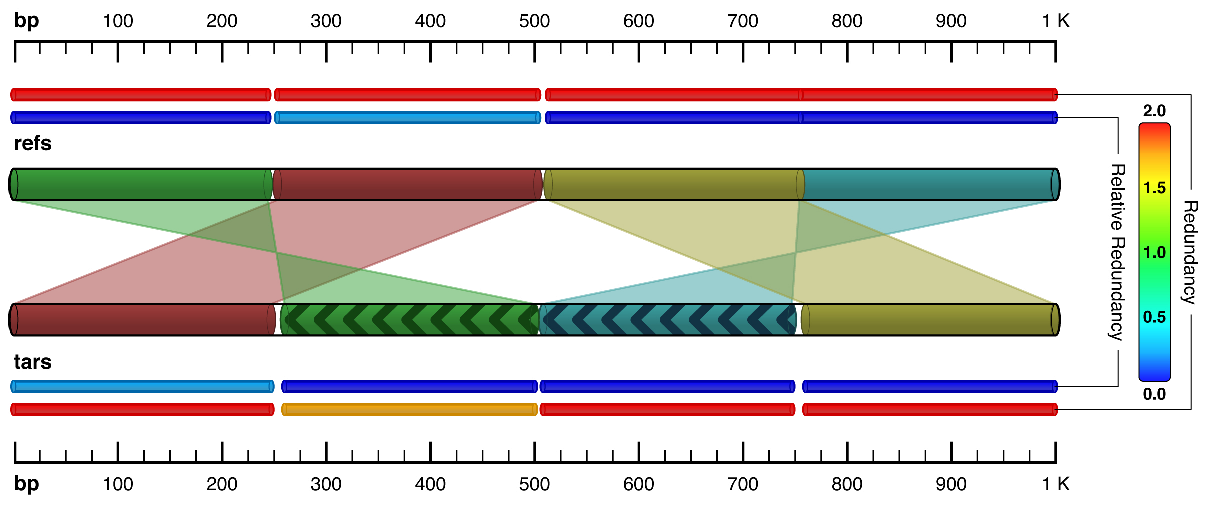
\includegraphics[width=\linewidth]{example.pdf}
  \caption{The result of running Smash++ on ...}
  \label{fig.example}
\end{figure}
\clearpage
%\balance
\refLineSpace    %%% Line spacing
\small
\addcontentsline{toc}{section}{\:\textbf{References}}
\bibliographystyle{IEEEtran}
\bibliography{ref}


\end{document}